\documentclass[aspectratio=169,xcolor=table]{beamer}
%aspcetratio >> 1610 169 149 54 43 32
%The themes:
%\usetheme[style=classic]{mharvellous}
%\usetheme[style=dark]{mharvellous}
%\usetheme[style=mracula]{mharvellous}
\usetheme[style=default]{mharvellous}
%*--------------------------------------------------
%\usepackage{helvet}
%*--------------------------------------------------
\usepackage{bibunits}  
%\setbeamertemplate{bibliography item}{[\theenumiv]}
\setbeamertemplate{bibliography item}{\insertbiblabel}
\defaultbibliography{bibliography}
%\defaultbibliographystyle{IEEEtran}
%\defaultbibliographystyle{amsalpha}
\defaultbibliographystyle{abntex2-alf}
%\bibliography{bibliography}
%\usepackage[backend=biber,style=alphabetic,citestyle=authoryear]{biblatex}
% \addbibresource{bibliography.bib}
%\usepackage{natbib}
\usepackage{bibentry}
%*--------------------------------------------------
\usepackage{lipsum}
\usepackage{epigraph}
\usepackage{graphicx}
\usepackage{multirow}
%\usepackage{enumitem}
\usepackage{array}
%\usepackage{multimedia}
\usepackage{media9}
%\usepackage{pdfpc-movie}
\usepackage{circledsteps}
\usepackage{listings}
\usepackage[normalem]{ulem}
%\usepackage{Sweave}
%\usepackage{xkeyval}
%\usepackage{palatino}
%\usepackage{pgfpages}
\usepackage{float}
%*--------------------------------------------------
\usepackage[timeinterval=1]{tdclock}
%\usepackage[font=Times,timeinterval=1, timeduration=200,resetatpages=all]{tdclock}
%\usepackage[font=Times,timeinterval=10, timeduration=2.0, timedeath=0, fillcolorwarningsecond=white!60!yellow,timewarningfirst=50,timewarningsecond=80,resetatpages=2]{tdclock}
%*--------------------------------------------------
\usepackage{url}
\usepackage{tabularx,booktabs}
\usepackage{threeparttable}
\usepackage[absolute, overlay]{textpos}
%*--------------------------------------------------
\usepackage{framed, color}
\usepackage[tikz]{bclogo}
\usepackage{spot}
\setspotlightcolor{red!50}
% %\setspotlightstyle{star, fill=red!50}
% %\setspotlightstyle{star points=7}
\usepackage{color,soul}
%\usepackage{xcolor}
\usepackage{tcolorbox}
\usepackage{xcolor}
\usepackage[export]{adjustbox}
\usepackage{verbatim}
\usetikzlibrary{trees,shapes,arrows}
\usepackage{fancyvrb}
\usepackage{float}
%*--------------------------------------------------
\usepackage{amsmath}
\usepackage{xfrac}
\usepackage{units}
\usepackage{ulem}
%*-------------------------------------------------------------------------------
%\newcolumntype{C}[1]{>{\centering\arraybackslash}m{#1}}
\newcolumntype{L}[1]{>{\raggedright\let\newline\\\arraybackslash\hspace{0pt}}m{#1}}
\newcolumntype{C}[1]{>{\centering\let\newline\\\arraybackslash\hspace{0pt}}m{#1}}
\newcolumntype{R}[1]{>{\raggedleft\let\newline\\\arraybackslash\hspace{0pt}}m{#1}}
%*-------------------------------------------------------------------------------
%\pgfpagesuselayout{2 on 1}[a4paper,border shrink=5mm]
%\setbeamertemplate{note page}[plain]
%\setbeameroption{show notes on second screen=bottom}
%*-------------------------------------------------------------------------------
\setbeameroption{hide notes}
%\setbeameroption{show only notes}
%\setbeameroption{show notes on second screen=right}
\setbeamertemplate{note page}{\pagecolor{yellow!5}\insertnote}
%*-------------------------------------------------------------------------------

%*-------------------------------------------------------------------------------
\title              {Título}
\subtitle           {Subtítulo}
\author             {Nome Sobrenome}
\email              {nome@site.com}
\advisor            {Orientador: Marco A. dos Reis}
\institute          {Robótica e Sistemas Autônomos, Senai Cimatec}
\date               {Mês de 202x}
% \ulogo        		{Template/logosenaicimatecnegativo}
% \ulogof             {Template/logosenaicimatec2020}
% \ulogoo        		{Template/rosa-logo}
% \ulistelement    	{Template/bullet-white}

%*-------------------------------------------------------------------------------
\graphicspath{{Source/pictures/}}
%*-------------------------------------------------------------------------------
\totalNoSlidesDisabled % To turn off the total number of slides in the footer. Comment this if you want the total number of slides in the footer
%*-------------------------------------------------------------------------------
\begin{document}
%*----------- COVER -------------------------------------------------------------
 \begin{frame}[t,plain]
%*----------- sound--------------------------------
    \includemedia[
        %width=1ex,
        %height=1ex,
        %activate=pageopen, 
        activate=onclick,
        deactivate=onclick,
        %passcontext,
        transparent,
        addresource=./Source/sounds/hip-hop.mp3,
        flashvars={
                    source=./Source/sounds/hip-hop.mp3
                    %&autoPlay=true
                    &autoRewind=true
                    &Play=2s
                    &repeat=always
                    %&Loop=true
        }
    ]
    {}{VPlayer.swf}
%*----------- start-page--------------------------
    \titlepage
    %*----------- notes-------------------------------
    \note[item]{Notes can help you to remember important information. Turn on the notes option.}
\end{frame}
%-
%*----------- SECTIONS ----------------------------------------------------------
%*----------- INTRODUÇÃO -------------------------------------------------------------
\begin{frame}[t]{Introdução} 
    \newcommand\vspaceintro{0.2cm}
    \transdissolve[duration=0.5]
    No Chile, até os anos 70 a agricultura era voltada, majoritariamente, ao fornecimento interno de produtos agrícolas não processados \cite{blueberryrecognition}\vspace{\vspaceintro}
    
    Atualmente, a agricultura é reponsável por 11\% do PIB (\$27 bilhões), representando 28\% do comércio e empregando 10\% da força de trabalho nacional\cite{ChilePIB:online} \vspace{\vspaceintro} 

    80\% das plantações de blueberry são do tipo "legacy blueberries"
    \vspace{-0.4cm}
    \begin{columns}[t]
        \column{.4\linewidth}
        \begin{center}
            %\centerline{
                \begin{figure}
                    %\roundpic[xshift=0cm,yshift=0cm]{5cm}{8cm}{dying-blueberry.jpg}
                    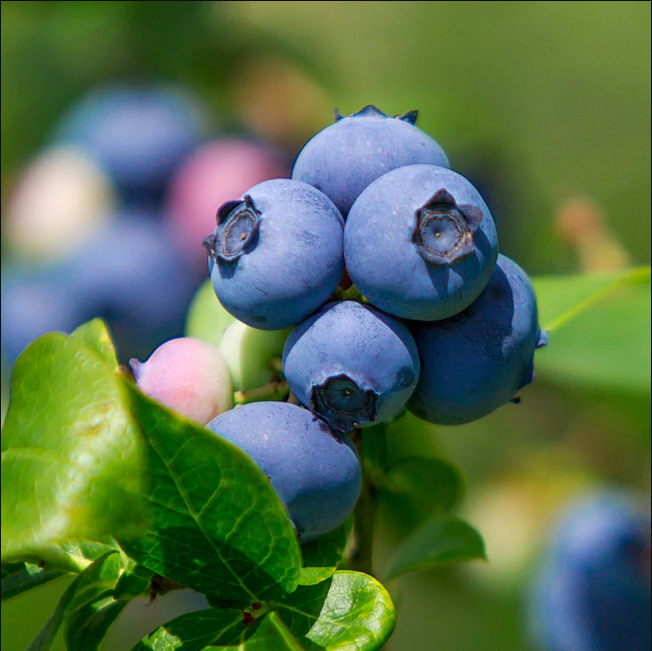
\includegraphics[width=0.5\textwidth]{blueberry-1.png}
                    %\caption{Pista de corrida \cite{agostini2007}}
                \end{figure}
            %}
        \end{center}

        \column{.4\linewidth}
        \begin{center}
            %\centerline{
                \begin{figure}
                    %\roundpic[xshift=0cm,yshift=0cm]{5cm}{8cm}{dying-blueberry.jpg}
                    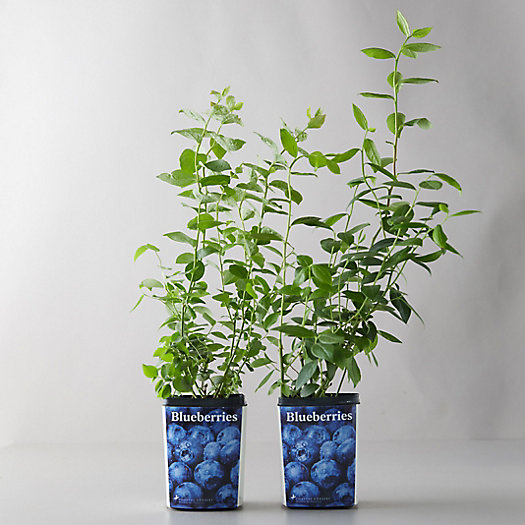
\includegraphics[width=0.5\textwidth]{blueberry-3.jpeg}
                    %\caption{Pista de corrida \cite{agostini2007}}
                \end{figure}
            %}
        \end{center}

        \column{.4\linewidth}
        \begin{center}
            %\centerline{
                \begin{figure}
                    %\roundpic[xshift=0cm,yshift=0cm]{5cm}{8cm}{dying-blueberry.jpg}
                    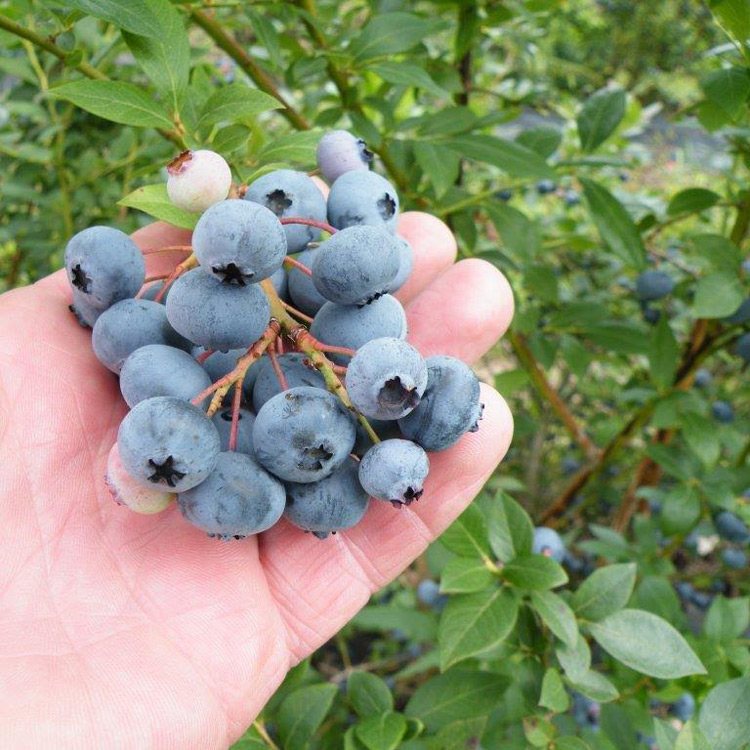
\includegraphics[width=0.5\textwidth]{blueberry-2.jpeg}
                    %\caption{Pista de corrida \cite{agostini2007}}
                \end{figure}
            %}
        \end{center}

    \end{columns}

    

%*----------- notes
    \note[item]{Notes can help you to remember important information. Turn on the notes option.}
\end{frame}
%-

%*----------- PROBLEMÁTICA -------------------------------------------------------------
\begin{frame}[t]{Problemática} 
    \transdissolve[duration=0.5]
    A agricultura chilena enfrenta os seguintes problemas:
    %\newline
        \begin{columns}[t]
            \column{.05\linewidth}
            \column{.4\linewidth}
                \begin{enumerate}
                    \item há previsões para o ano de 2030 sobre um abondono significativo dos trabalhadores na agricultura
                    \item no estágio de enraizamento durante as estações críticas ocorrem perdas superiores a 50\% dos brotos
                \end{enumerate}
            \column{.6\linewidth}
            \vspace{-0.5cm}
            \begin{center}
                \begin{figure}
                    \caption{Legacy Blueberry Seca}
                    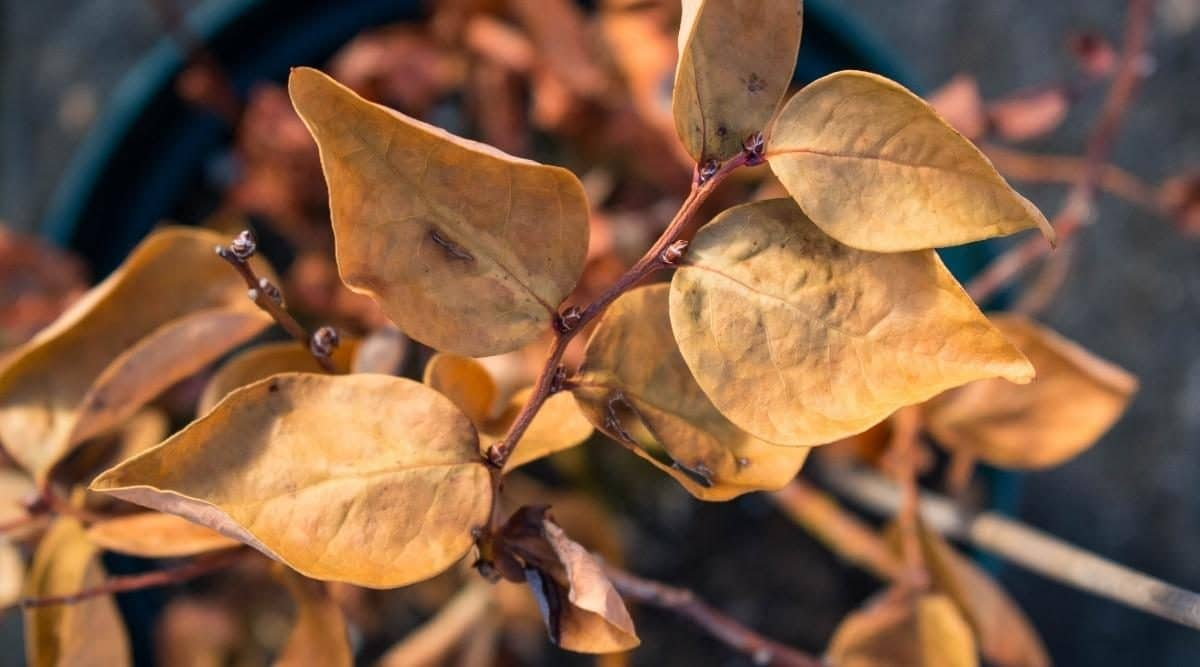
\includegraphics[width=0.7\textwidth]{dying-blueberry.jpg}
                \end{figure}
            \end{center}
        \end{columns}
%*----------- notes
    \note[item]{Notes can help you to remember important information. Turn on the notes option.}
\end{frame}
%-
%*----------- SLIDE -------------------------------------------------------------
\begin{frame}[c]{A tropa dos quatro incríveis}
    %\transboxin[duration=1,direction=30]
    A simulação deverá ser desenvolvida com 4 unidades Darwin-OP, comumente esta unidade é utilizada para desafios em competições de robótica.
    \newline

    A tropa será composta por 4 Darwin-OP, e deverá realizar duas missões:
    \begin{itemize}
        \item marchar em forma unida em linha;
        \item realizar corrida de revezamento.
    \end{itemize}

    \begin{figure}
        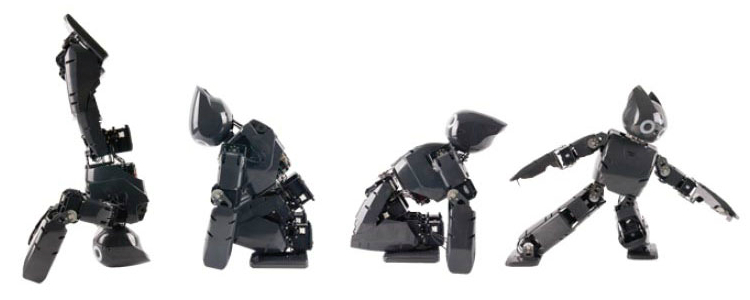
\includegraphics[trim = 0 20 0 50, clip, width=0.8\textwidth]{darwin-op-sequencia}
        %\caption{.}
    \end{figure}
%*----------- notes
    \note[item]{Notes can help you to remember important information. Turn on the notes option.}
\end{frame}
%-
%*----------- SLIDE -------------------------------------------------------------
\begin{frame}[t]{Algumas regras}
    \begin{itemize}
        \item A marcha deverá ser realizada diante de um percurso de 2 metros.
        \item A marcha e a corrida de revezamento deverão serem realizadas numa pista de corrida;
        \item A corrida deverá ser realizada numa pista de 8 metros;
        \item Cada Darwin-OP deverá percorrer 2 metros para realizar o revezamento;
        \item A região de revezamento deverá ser uma área de até 0.4 metros;
        \item O conceito para o revezamento será o de alinhar-se os dois Darwin-OP durante até 15 segundos a uma distância de no máximo 0.2 metros entre ambos, ou seja será considerado passagem de bastão quando os dois Darwin-OP passarem 15 segundos com movimentos sincronizados a uma distância máxima de 0.2 metros dentro da região de revezamento;
        \item A pista de corrida deverá ser considerada analogamente a uma pista real;
        \item A lateral da pista deverá ter lados de 2 metros;
        \item Considerar sempre os critérios de uma corrida de revezamento.
    \end{itemize}
   
    % \begin{columns}[t]
    %     \column{.45\textwidth}
    %         detalhar sistemas em subconjuntos\\
    %         listar possíveis modos de falhas\\
    %         analisar cada modo de falha, juntamente com suas possíveis causas e sintomas
    %     \column{.45\textwidth}
    %         estimar os efeitos de cada modo de falhas\\
    %         estimar a criticidade de cada efeito\\
    %         identificar ações para minimizar falhas
    % \end{columns}
%*----------- notes
    \note[item]{Notes can help you to remember important information. Turn on the notes option.}
\end{frame}
%-
%*----------- SLIDE -------------------------------------------------------------
\begin{frame}[c]{A pista}
    \begin{figure}
        %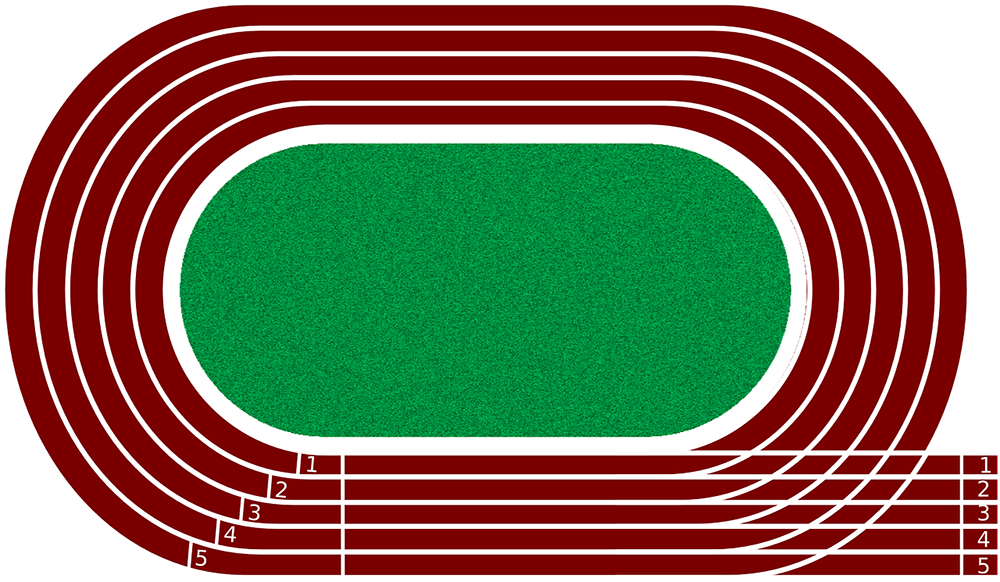
\includegraphics[width=0.7\textwidth]{pista_corrida}
       
        \roundpic[xshift=0cm,yshift=0cm]{3cm}{7cm}{pista_corrida}
          
        \caption{Formato de um pista de corrida.\cite{agostini2007}}
    \end{figure}
%*----------- notes
    \note[item]{Notes can help you to remember important information. Turn on the notes option.}
\end{frame}
%-
%*----------- SLIDE -------------------------------------------------------------
\begin{frame}[t]{Metodologia - Avaliação do modelo}
    Para analisar o modelo criado, os autores adotadaram quatro métricas 
    \vspace{0.4cm}

    O parâmetro \textbf{\textit{"Accuracy"}}  representa a fração das predições feitas corretamente
    \vspace{0.4cm}

    A \textbf{\textit{"Precision"}} é a razão entre as predições verdadeiras corretas dentre todas as predições verdadeiras, corretas ou não 
    \begin{table}[]
        \vspace{0.8cm}
        \centering
        \begin{tabular}{ll}
            \begin{math} Accuracy = \frac{Number\,of\,correct\,predictions}{Total\,number\,of\,predictions} \end{math} 
            &
            \begin{math} Precision = \frac{True\,Positive}{True\,Positive + False\,Negative} \end{math} 
        \end{tabular}
    \end{table}
    
%*----------- notes
    \note[item]{Notes can help you to remember important information. Turn on the notes option.}
\end{frame}

%*----------- SLIDE -------------------------------------------------------------
\begin{frame}[t]{Metodologia - Avaliação do modelo}
    O parâmetro \textbf{\textit{"Recall"}} é a habilidade do modelo de encontrar os verdadeiros positivos
    \vspace{0.4cm}
    
    A \pmb{"\begin{math} F_1Score \end{math}"} é a média harmônica pondera entre os parâmetros \textit{"Precision"} e \textit{"Recall"}
    \begin{table}[]
        \vspace{0.8cm}
        \centering
        \begin{tabular}{ll}
            \begin{math} Recall = \frac{True\,Positive}{True\,Positive + False\,Negative} \end{math}
            &
            \begin{math} F_1Score = 2\cdot\frac{Precision \cdot Recall}{Precision + Recall} \end{math}
        \end{tabular}
    \end{table}
    
%*----------- notes
    \note[item]{Notes can help you to remember important information. Turn on the notes option.}
\end{frame}
% FALTA: contexto(onde e como), mapa, solução
%*----------- SLIDE -------------------------------------------------------------
\begin{frame}[t]{Resultados}
    \begin{columns}
        \column{0.5\textwidth}
            \vspace{0.4cm}
            \begin{figure}
                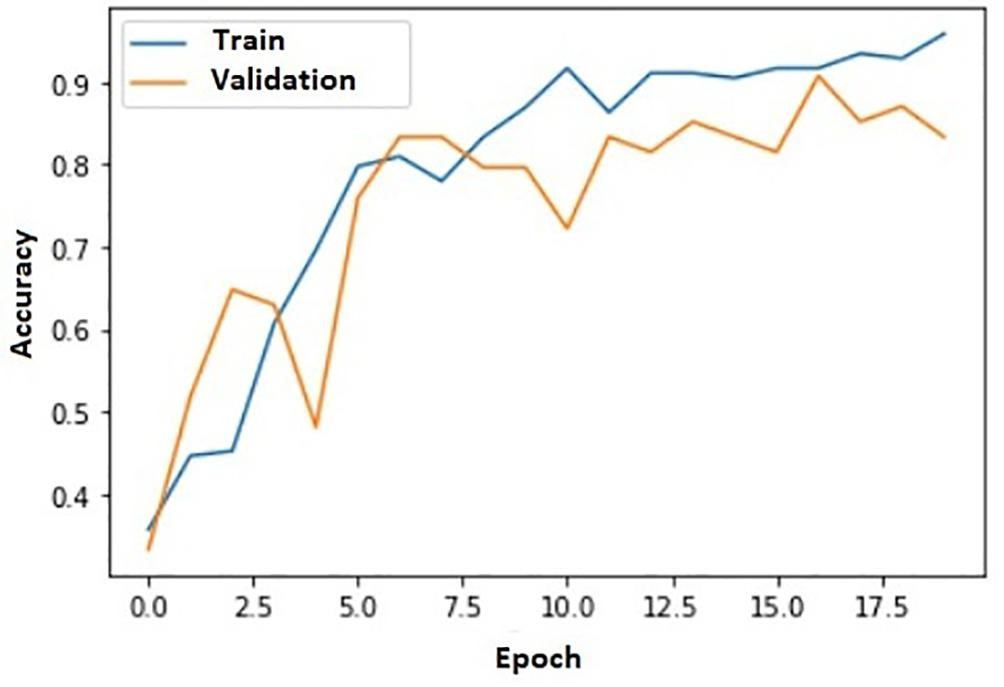
\includegraphics[width=.9\textwidth]{grafico-accuracy.jpg}
            \end{figure}
        \column{.5\textwidth}
        \begin{center}
            \vspace{0.4cm}
            \begin{figure}
                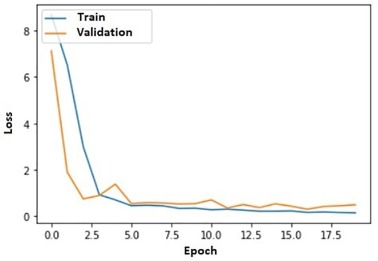
\includegraphics[width=.9\textwidth]{grafico-perdas.jpg}
            \end{figure}    
        \end{center}
            
    \end{columns}
%*----------- notes
    \note[item]{Notes can help you to remember important information. Turn on the notes option.}
\end{frame}

%*----------- SLIDE -------------------------------------------------------------
\begin{frame}[t]{Resultados}
    Matriz de confusão do modelo preditivo
    \begin{table}[]
        \centering
        \begin{tabular}{cccc}
        \hline
        \multirow{2}{*}{\vspace{-0.5cm}\textit{Real}}     & \multicolumn{3}{c}{\textit{Predição}}                                                                                                                                              \\ \cline{2-4} 
                                        & \textit{\begin{tabular}[c]{@{}c@{}}Bandeja com plantas\\ vivas\end{tabular}} & \textit{\begin{tabular}[c]{@{}c@{}}Bandeja sem plantas\\ vivas\end{tabular}} & \textit{Sem bandeja} \\ \hline
        \textit{Bandeja com plantas vivas} & 9                                                                            & 1                                                                            & 0                    \\
        \textit{Bandeja sem plantas vivas} & 3                                                                            & 11                                                                           & 1                    \\
        \textit{Sem bandeja}               & 0                                                                            & 0                                                                            & 11                   \\ \hline
        \end{tabular}
    \end{table}
%*----------- notes
    \note[item]{Notes can help you to remember important information. Turn on the notes option.}
\end{frame}

%*----------- SLIDE -------------------------------------------------------------
\begin{frame}[t]{Resultados}
    Resultados obtidos para o modelo de predição (médias em negrito)
    \begin{table}[]
        \centering
        \begin{tabular}{cccc}
        \hline
        \multirow{2}{*}{\textit{Classe}}   & \multicolumn{3}{c}{\textit{Métricas}}                    \\ \cline{2-4} 
                                        & \textit{Precision} & \textit{Recall} & \textit{F1 Score} \\ \hline
        \textit{Bandeja com plantas vivas} & 0.75               & 0.90            & 0.82              \\
        \textit{Bandeja sem plantas vivas} & 0.92               & 0.73            & 0.81              \\
        Sem bandeja                        & 0.92               & 1.00            & 0.96              \\
        \textit{\textbf{Média}}            & \textbf{0.86}      & \textbf{0.88}   & \textbf{0.86}     \\ \hline
        \end{tabular}
    \end{table}
%*----------- notes
    \note[item]{Notes can help you to remember important information. Turn on the notes option.}
\end{frame}
%----------------------------------------------------SLIDE------------------
 \begin{frame}[t, allowframebreaks]{References}
 %\frametitle{References}
%\begin{frame}{Reference}
    %\transboxin[duration=1,direction=30]

    % \begin{bibunit}[plain]
    % \cite{guangyi2018research}.
    % %\cite{kanakia2012}
    % %\cite{agostini2007}
    % %\cite{azuma1997survey}
    % \cite{Buss2005}
  
    % \putbib
    % \end{bibunit}
  
    %\bibliographystyle{IEEEtran}
    %\bibliographystyle{IEEEtranS}
    %\bibliographystyle{IEEEbib}
    \bibliographystyle{abntex2-alf}
    %\bibliographystyle{abntex2-num}
    %\bibliographystyle{abnt-alf}
    \bibliography{bibliography} 
    %\putbib

%*----------- notes
    %\note[item]{Notes can help you to remember important information. Turn on the notes option.}
\end{frame}
%
%-
%*----------- SLIDE-BACKUP ------------------------------------------------------
% \backupbegin
% %
% \begin{frame}{Backup}
%     Test
% %*----------- notes-------------------------------
% \note{Notes can help you to remember important information. Turn on the notes option.}
% \end{frame}
% %-
% \backupend
% %-
%*----------- QUESTIONS ---------------------------------------------------------
\begin{frame}[c,plain]
    \lastpage{
        \begin{center}   
            {\usebeamerfont{title} Questions?}\\[3ex] 
            %\hspace{1.5cm} 
            marco.a.reis@google.com
        \end{center}
    }
    
    %*----------- notes---------------------------------
    \note[item]{Notes can help you to remember important information. Turn on the notes option.}
\end{frame}
%*-------------------------------------------------------------------------------
\end{document}